\subsubsection{Arbitrage as a violation metric}
\label{cfc/app:arbitrage}

\rebuttal{For the following definition we use a slightly more general notation than in the main body, to convey that our methods could be generalized beyond binary forecasting questions. }

\begin{notation*}

    \rebuttal{Let $\ForecastingQuestions$ denote the set of forecasting questions we are interested in, $\Resolutions$ denote the set of possible outcomes/resolutions for an individual question, and $\Forecasts$ denote the set of probability distributions on $\Resolutions$. A \emph{Forecaster} is a map $\Forecaster:\ForecastingQuestions\to\Forecasts$. For conditional questions that can resolve to $\none$, we also have optional resolutions $\ResolutionsOpt:=\Resolutions\cup\{\none\}=\boolsopt$.}
\end{notation*}


The arbitrage metric may be seen as being motivated by Dutch Book Arguments for probabilistic consistency rules (see e.g. \cite{vinebergDutchBookArguments2022}). Imagine the forecaster's predictions $\Forecaster(x_1),\dots\Forecaster(x_n)$ were prices offered by a bookie on prediction markets for sentences $x_1,\dots x_n$. If these probabilities are inconsistent, then there are bets that an arbitrageur can make that guarantee a profit in \emph{all possible (consistent) worlds regardless of the individual outcomes}. For example, if $x_1,x_2$ are two sentences such that $x_1\iff x_2$, but the bookie prices $\Forecaster(x_1)<\Forecaster(x_2)$, then an arbitrageur can simply buy $x_1$ and sell $x_2$ to make a risk-free profit.

However, if the bookie never changes their prices in response to trades, the arbitrageur can make an infinite amount of profit with its strategy. This is neither realistic nor useful for creating a metric to measure inconsistency. Instead, we turn to \emph{market scoring rules}, introduced in \citet{hansonLogarithmicMarketScoring2002}), where the bookie is a \emph{market-maker} who updates market prices in a way that ensures that the reward for moving the market price of a sentence that resolves True from $p_0$ to $p'$ is given by a \emph{proper scoring rule} \footnote{A proper scoring rule \citep{savageElicitationPersonalProbabilities1971}, is one that incentivizes honest reporting of probabilities: widely used proper scoring rules include the Brier score $(1-p)^2$ and the logarithmic scoring rule $-\log p$.} $s(p')-s(p_0)$. We then define our inconsistency metric to be the minimum profit an arbitrageur can guarantee against such a market-maker, if the latter offers inconsistent probabilities $\Forecaster(x_1),\dots\Forecaster(x_n)$.

\begin{definition}[Arbitrage-based Violation Metric]
    Let $\Relation:\ForecastingQuestions^n\to\bools$ be an n-ary relation such that $\Relation(\Resolution(x_1), \dots \Resolution(x_n))$ is satisfied by the ground-truth resolutions $\Resolution:\ForecastingQuestions\to\Resolutions$ for all tuples $(x_1,\dots x_n)$. \footnote{This is well-defined because resolutions can be taken as a subset $\Resolutions\subseteq\ForecastingQuestions$, by treating them as forecasting questions that always resolve to themselves by definition. For example, the forecasting question $\top$ is always worth \$1 and the forecasting question $\bot$ is always worth \$0.} Let $s:\ForecastingQuestions\times\Resolutions\times[0,1]\to\Reals$ be a proper scoring rule that gives the score earned based on the probability assigned to the true resolution, e.g. $s(x,\Resolution,p(\Resolution))=\log p(\Resolution)$. Let $(x_1,\dots x_n)\in\ForecastingQuestions^n$ be a question tuple, and denote $\ResolutionsVec:=\{\resolutionvec\in\ResolutionsOpt^n\mid\Relation(\resolutionvec)\}$ the set of possible consistent resolutions (including $\none$ resolutions) of this tuple. Then for forecasts $(\Forecaster(x_1),\dots\Forecaster(x_n))$ the arbitraged forecasts $\Arbitrageur(\Forecaster(x_1),\dots\Forecaster(x_n))=(p_1\dots p_n)$ and the minimum guaranteed profit of the arbitrageur $\Violation(\Forecaster(x_1),\dots\Forecaster(x_n))$ are given by:

    \begin{equation}
        \argmaxmax_{\consp\in\Forecasts^n}
        \min_{\resolutionvec\in\ResolutionsVec}
        \sum_{i=1}^n
        %\sum_{\Resolution\in\Resolutions}
        \score{x_i, \resolutionvec_i, p_i(\resolutionvec_i)}
        - \score{x_i, \resolutionvec_i, \Forecaster(x_i)(\resolutionvec_i)}%\Indicator{\omega_i=\Resolution}
        \label{eq:arbitrage}
    \end{equation}
    Where by convention, any score on a resolution $\resolutionvec_i=\none$ is taken to be 0.
    \label{def:arbitrage}
\end{definition}

Definition~\ref{def:arbitrage} is presented in full generality: $\consp$ and $\Forecaster(x_i)$ here are \emph{probability distributions} on $\Resolutions$. Breaking it down: each $\score{x_i, \resolutionvec_i, p_i(\resolutionvec_i)}- \score{x_i, \resolutionvec_i, \Forecaster(x_i)(\resolutionvec_i)}$ gives the arbitrageur's profit on the market for question $x_i$, given that it resolves $\resolutionvec_i$. The profit is summed across all markets in the tuple, and then minimized over all consistent worlds; this minimum is maximized across all possible arbitrageur bets.

It is helpful to explicitly state Eq~\ref{eq:arbitrage} in the case of binary forecasting questions, as follows.

\begin{equation}
    \argmaxmax_{\consp\in[0,1]^n} \min_{\omega\in\Omega} \sum_{i=1}^n \left(\score{\consp_i}-\score{\Forecaster(x_i)}\right)\Indicator{\omega(i)=\top} + \left(\score{1-\consp_i}-\score{1-\Forecaster(x_i)}\right)\Indicator{\omega(i)=\bot}
    \label{eq:arbitrage_}
\end{equation}



% \NewDocumentCommand{\score}{m}{\ensuremath{s\left(#1\right)}}
% \NewDocumentCommand{\consp}{}{p}
% \NewDocumentCommand{\argmaxmax}{}{\mathop{(\argmax,\max)}}

% If an arbitrageur could trade
% inconsistent probabilities offered on the market for arbitrary amounts of money, the profit would be infinite.
% This is neither realistic nor useful.
% In real-world markets (both prediction and financial),
% the mechanism that resolves this is
% a \emph{market maker}: an entity that accepts trades at market probabilities, but updates them slightly on every trade.

% A proper scoring rule, introduced in \cite{savageElicitationPersonalProbabilities1971}, is one that incentivizes honest reporting of probabilities.
% \citet{hansonLogarithmicMarketScoring2002} shows that the \emph{logarithmic scoring rule} has useful properties for modeling the market maker.

% \todo{Manyu: write here. or maybe it's better that Daniel writes this so he understands

% TODO explain how we get the log thing.
% }

% The arbitrage metric may be seen as being motivated by Dutch Book Arguments for probabilistic consistency rules (see e.g. \cite{vinebergDutchBookArguments2022}). The idea is as follows: imagine the forecaster's predictions $\Forecaster(P_1),\dots\Forecaster(P_n)$ were prices offered by a bookie on prediction markets for sentences $P_1,\dots P_n$. If these probabilities are inconsistent, then there are bets that an arbitrageur can make that guarantee a profit in \emph{all possible (consistent) worlds regardless of the individual outcomes}. For example, if $P,Q$ are two sentences such that $P\iff Q$, but the bookie prices $\Forecaster(P)<\Forecaster(Q)$, then an arbitrageur can simply buy $P$ and sell $Q$ to make a risk-free profit.

% If the bookie never changes their prices in response to trades, the arbitrageur can make an infinite amount of profit with its strategy. This is neither realistic nor useful for creating a metric for measuring inconsistency. Instead, we suppose the bookie (or ``market-maker'') updates his prices in accordance with a \emph{market scoring rule} (introduced in \citet{hansonLogarithmicMarketScoring2002}). In particular, \citet{hansonLogarithmicMarketScoring2002} shows that it is possible for the market-maker to update its prices so that the reward for moving the market price of a sentence that resolves True from $p_0$ to $p'$ is given by a \emph{proper scoring rule} $s(p',p_0)$, e.g. the logarithmic scoring rule $\log(p')-\log(p_0)$.

% We regard the forecaster's probabilities $\Forecaster(x_1),\Forecaster(x_2), \ldots$ as the spot prices offered on a prediction market with a proper scoring rule (taken to be $s(p)=\log(p)$ by default)
% for $x_1,x_2$, etc.
% %
% If these forecasts are inconsistent, then an arbitrageur can profit from bringing the market prices to consistency. In particular, there is a minimum guaranteed risk-free profit, called \emph{arbitrage}, that the forecaster can be guaranteed to obtain regardless of the outcome of $x_1,x_2$ etc., i.e. without taking a position on the base outcomes. This minimum guaranteed arbitrage can be taken to be a consistency violation metric.

% \begin{definition}[Arbitrage-based Violation Metric]
%     Let $\Relation:\ForecastingQuestions^n\to\bools$ be an n-ary relation such that $\Relation(\Resolution(x_1), \dots \Resolution(x_n))$ is satisfied by the ground-truth resolutions $\Resolution:\ForecastingQuestions\to\Resolutions$ for all tuples $(x_1,\dots x_n)$. \footnote{This is well-defined because resolutions can be taken as a subset $\Resolutions\subseteq\ForecastingQuestions$, by treating them as forecasting questions that always resolve to themselves by definition. For example, the forecasting question $\top$ is always worth \$1 and the forecasting question $\bot$ is always worth \$0.} Let $s:\ForecastingQuestions\times\Resolutions\times[0,1]\to\Reals$ be a proper scoring rule that gives the score earned based on the probability assigned to the true resolution, e.g. $s(P,\Resolution,p(\Resolution))=\log p(\Resolution)$. Let $(x_1,\dots x_n)\in\ForecastingQuestions^n$ be a question tuple, and denote $\ResolutionsVec:=\{\resolutionvec\in\ResolutionsOpt^n\mid\Relation(\resolutionvec)\}$ the set of possible consistent resolutions (including $\none$ resolutions \todo{this requires its own clarifying paragraph or a subsection, with an example}) of this tuple. Then for forecasts $(\Forecaster(x_1),\dots\Forecaster(x_n))$ the arbitraged forecasts $(p_1\dots p_n)$ and the minimum guaranteed profit of the arbitrageur $\Violation(\Forecaster(x_1),\dots\Forecaster(x_n))$ are given by:

%     \begin{equation}
%         \argmaxmax_{\consp\in\Forecasts^n}
%         \min_{\resolutionvec\in\ResolutionsVec}
%         \sum_{i=1}^n
%         %\sum_{\Resolution\in\Resolutions}
%         \score{x_i, \resolutionvec_i, p_i(\resolutionvec_i)}
%         - \score{x_i, \resolutionvec_i, \Forecaster(x_i)(\resolutionvec_i)}%\Indicator{\omega_i=\Resolution}
%         \label{eq:arbitrage}
%     \end{equation}
%     Where by convention, any score on a resolution $\resolutionvec_i=\none$ is taken to be 0.
%     \label{def:arbitrage}
% \end{definition}

% %(The $\argmaxmax$ may also be taken over only consistent $p$, i.e. $p$ satisfying $\CCheck(p)$, but doesn't make a difference because the max will always be for a consistent $p$ anyway since otherwise you could arbitrage further.) We will work this out in detail as an example for ParaphraseChecker for understanding, then simply substitute

% Definition~\ref{def:arbitrage} is presented in full generality: $\consp$ and $\Forecaster(x_i)$ here are \emph{probability distributions} on $\Resolutions$. Breaking it down: each $\score{x_i, \resolutionvec_i, p_i(\resolutionvec_i)}- \score{x_i, \resolutionvec_i, \Forecaster(x_i)(\resolutionvec_w)}$ gives the arbitrageur's profit on the market for question $x_i$, given that it resolves $\resolutionvec_i$. The profit is summed across all markets in the tuple, and then minimized over all consistent worlds; this minimum is maximized across all possible arbitrageur bets.

% It is helpful to explicitly state \Cref{eq:arbitrage} in the case of binary forecasting questions, as follows.

% \begin{equation}
%     \argmaxmax_{\consp\in[0,1]^n} \min_{\omega\in\Omega} \sum_{i=1}^n \left(\score{\consp_i}-\score{\Forecaster(x_i)}\right)\Indicator{\omega(i)=\top} + \left(\score{1-\consp_i}-\score{1-\Forecaster(x_i)}\right)\Indicator{\omega(i)=\bot}
%     \label{eq:arbitrage_}
% \end{equation}

We will illustrate our violation metric with three specific examples, for \ParaphraseChecker{}, \NegChecker{} and \CondChecker{}. For other consistency checks, the math becomes too convoluted and we use a numerical method in our project code.

\subsubsubsection{ParaphraseChecker}
\label{apps:checks-paraphrase}

\RenewDocumentCommand{\priceP}{}{\Forecaster(P)}
\RenewDocumentCommand{\priceQ}{}{\Forecaster(Q)}

Let $P$ and $Q$ be equivalent sentences, and suppose that the forecaster produces forecasts $\priceP$ and $\priceQ$. A trader who instead brings prices to $\Forecaster'(P)=\Forecaster'(Q)=\consp$ for both questions earns a combined profit on both questions:

\begin{equation}
\begin{cases}
    \score{\consp}-\score{\priceP}+\score{\consp}-\score{\priceQ} & \text{if } P \\
    \score{1-\consp}-\score{1-\priceP}+\score{1-\consp}-\score{1-\priceQ} & \text{if } \lnot P
\end{cases}
\label{eq:profit-paraphrase}
\end{equation}

For this first example, we can graph this profit as a function of $\consp$ for illustration, shown in Fig.~\ref{fig:profit-paraphrase} -- demonstrating that any $\consp\in(0.529,0.576)$ is profitable for the arbitrageur, and further that the arbitrageur can \textit{guarantee} a minimum profit of $0.095$ regardless of the outcome of $P$ by choosing the consistent probability $\consp=0.555$.

\begin{figure}
\centering
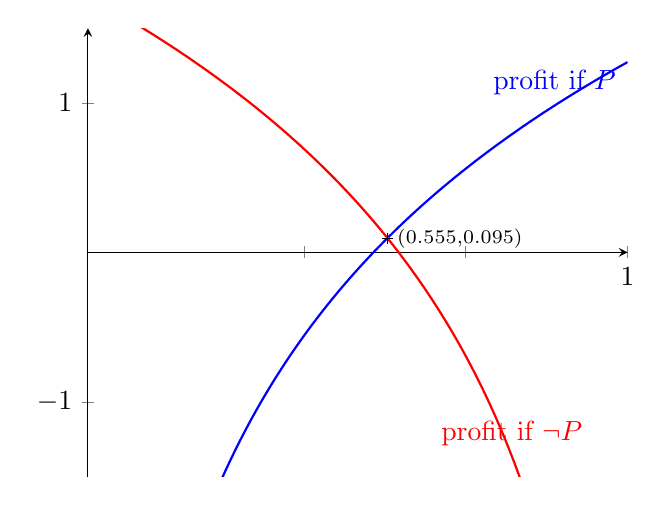
\begin{tikzpicture}
    \begin{axis}[
        axis lines=middle,
        xlabel=$\consp$,
        ylabel={},
        xmin=0, xmax=1,
        ymin=-1.5, ymax=1.5,
        %legend pos=outer north east,
        %clip=false,
        domain=0:1,
        samples=200,
        unbounded coords=jump, % Handling log(0) gracefully
        xtick={0, 0.4,0.7, 1.0},
        xticklabels={$0$,$\priceQ$, $\priceP$, $1$}
    ]
    \pgfmathdeclarefunction{s}{1}{\pgfmathparse{ln(#1)}}
    \addplot[blue, thick] {s(x) - s(0.7) + s(x) - s(0.4)} node[pos=0.97, above] {profit if $P$};
    \addplot[red, thick] {s(1-x) - s(1-0.7) + s(1-x) - s(1-0.4)} node[pos=0.15, above]{profit if $\lnot P$};

    %\legend{profit if $P$, profit if $\lnot P$}
    \addplot[only marks, mark=+, mark options={fill=black}] coordinates {(0.555, 0.095)}; % (0.5292,0) (0.5757,0)
    \node at (axis cs: 0.555, 0.095) [anchor=west] {$\scriptstyle{(0.555,0.095)}$};
    % \node at (axis cs: 0.5292, 0) [anchor=north]{$\scriptstyle{0.529}$};
    % \node at (axis cs: 0.5757, 0) [anchor=north]{$\scriptstyle{0.576}$};
    % \node at (axis cs: 0.7, 0) [anchor=south] {$P$};
    % \node at (axis cs: 0.4, 0) [anchor=south] {$Q$};
    \end{axis}
\end{tikzpicture}
\caption{Profit earned by the arbitrageur in case of inconsistency over ParaphraseChecker, taking $s(p)=\log(p)$ and $\priceP,\priceQ=0.7,0.4$ in \eqref{eq:profit-paraphrase}.}
\label{fig:profit-paraphrase}.
\end{figure}
% https://www.desmos.com/calculator/5kt8dkvr1e
% https://www.desmos.com/calculator/0fyuwmoasf

We may compute this intersection analytically:

\begin{align*}
    \score{\consp}-\score{\priceP}+\score{\consp}-\score{\priceQ} &=
    \score{1-\consp}-\score{1-\priceP}+\score{1-\consp}-\score{1-\priceQ} \\
    2\log\frac{\consp}{1-\consp}&=\log\frac{\priceP\priceQ}{(1-\priceP)(1-\priceQ)} \\
    \consp &= \frac{\sqrt{\priceP\priceQ}}{\sqrt{\priceP\priceQ}+\sqrt{(1-\priceP)(1-\priceQ)}} \\
\end{align*}

Substituting this back into either expression in \eqref{eq:profit-paraphrase} we get the expression for the arbitrage:

\begin{equation}
\Violation(\priceP,\priceQ)=-2\log\left(\sqrt{\priceP\priceQ}+\sqrt{(1-\priceP)(1-\priceQ)}\right)
\label{eq:arbitrage-paraphrase}
\end{equation}

As a bonus, this can straightforwardly be extended to the multi-question paraphrasing check: $(P_1\iff\dots\iff P_n)\implies(\Forecaster(P_1)=\dots=\Forecaster(P_n))$. Here the corresponding possible profits are:

\begin{equation}
\begin{cases}
    n\score{\consp}-\sum{\score{\Forecaster(P_i)}} & \text{if } P \\
    n\score{1-\consp}-\sum{\score{1-\Forecaster(P_i)}} & \text{if } \lnot P
\end{cases}
\label{eq:profit-paraphrase-multi}
\end{equation}

Equating them and solving for $\consp$, we get:

\begin{equation}
    \log\frac{p}{1-p}=\frac1n\sum_i\log\frac{\Forecaster(P_i)}{1-\Forecaster(P_i)}
    \label{eq:logodds-paraphrase-multi}
\end{equation}

\begin{equation}
    p=\frac{\Delta}{\Delta+1}
    \text{ where }
    \Delta=\left[\prod_i\frac{\Forecaster(P_i)}{1-\Forecaster(P_i)}\right]^{1/n}
    \label{eq:prob-paraphrase-multi}
\end{equation}

Observe that the arbitraged probability is simply the arithmetic mean in log-odds space! One may wonder if the violaton is some kind of variance measure in log-odds space, but this does not seem to be the case:

\begin{equation}
    \Violation(\Forecaster(P_1),\dots\Forecaster(P_n))=-n\log\left[
    \left(\prod\Forecaster(P_i)\right)^{1/n} +
    \left(\prod(1-\Forecaster(P_i))\right)^{1/n}
    \right]
    \label{eq:violation-paraphrase-multi}
\end{equation}

\subsubsubsection{NegChecker}
\label{apps:arbitrage-neg}

\NewDocumentCommand{\pricenotP}{}{\Forecaster(\lnot P)}

Suppose the forecaster produces forecasts $\Forecaster(P)$ and $\Forecaster(\lnot P)$. A trader who instead brings prices to $\Forecaster'(P)=\consp$, $\Forecaster'(\lnot P)=1-\consp$ earns a combined profit on both questions:

\begin{equation}
\begin{cases}
    \score{\consp}-\score{\priceP}+\score{\consp}-\score{1-\pricenotP} & \text{if } P \\
    \score{1-\consp}-\score{1-\priceP}+\score{1-\consp}-\score{\pricenotP} & \text{if } \lnot P
\end{cases}
\label{eq:profit-neg}
\end{equation}

Equating them and solving as before,

\begin{align*}
    2\log\frac{\consp}{1-\consp} &=
    \log\frac{\priceP(1-\pricenotP)}{(1-\priceP)\pricenotP} \\
    \consp &=
    \frac{\sqrt{\priceP(1-\pricenotP)}}{\sqrt{\priceP(1-\pricenotP)}+\sqrt{(1-\priceP)\pricenotP}} \\
\end{align*}

Substituting into \eqref{eq:profit-neg}, we get:

\begin{equation}
    \Violation(\priceP,\pricenotP)=-2\log\left(\sqrt{\priceP(1-\pricenotP)}+\sqrt{(1-\priceP)\pricenotP}\right)
\end{equation}

The similarity of these results to \ParaphraseChecker{} is suggestive: both the arbitraged probability and the violation for \NegChecker{} can be derived from \ParaphraseChecker{} simply replacing $\priceQ$ with $1-\pricenotP$, seeing the latter as the ``probability implied for $P$ by $\lnot P$''.
This raises the natural question: Can \emph{all} consistency checks be reduced to the case of \ParaphraseChecker{} arbitraging $\Forecaster(P)$ against an ``implied probability'' for $P$?

However, as we will see, \CondChecker{} shows that this approach does not always hold. Its violation expression depends on more than just $\Forecaster(P)$ and $\Forecaster(P\land Q)/\Forecaster(Q\mid P)$, so there is no single, neat interpretation akin to “arithmetic mean in the log-odds space.”

\subsubsubsection{CondChecker}

\NewDocumentCommand{\priceQgivenP}{}{\Forecaster(Q\mid P)}
\NewDocumentCommand{\pricePandQ}{}{\Forecaster(P\land Q)}
\NewDocumentCommand{\consq}{}{q}

Suppose the forecaster produces forecasts $\priceP$, $\priceQgivenP$, $\pricePandQ$. The possible outcomes $\Omega$ are $(P,Q\mid P,P\land Q)\mapsto$ $(\top,\top,\top)$, $(\top,\bot,\bot)$, $(\bot,\none,\bot)$. Consider an arbitrageur who makes bets $\Forecaster'(P)=\consp$, $\Forecaster'(Q\mid P)=\consq$, $\Forecaster'(P\land Q)=\consp\consq$.

In each outcome:

\begin{equation}
\begin{cases}
\score{\consp}-\score{\priceP}+\score{\consq}-\score{\priceQgivenP}+\score{\consp\consq}-\score{\pricePandQ}
& \mathrm{if } P,Q\\
\score{\consp}-\score{\priceP}+\score{1-\consq}-\score{1-\priceQgivenP}+\score{1-\consp\consq}-\score{1-\pricePandQ}
& \mathrm{if } P,\lnot Q\\
\score{1-\consp}-\score{1-\priceP}+\score{1-\consp\consq}-\score{1-\pricePandQ}
& \mathrm{if } \lnot P
\end{cases}
\label{eq:profit-cond}
\end{equation}

Equating these and rearranging:

\begin{equation*}
    \begin{cases}
    \frac{1-\consp}{\consp (1-\consq)} = \frac{1-\priceP}{\priceP(1-\priceQgivenP)} =: A\\
    \frac{1-\consq}{\consq}\frac{1-\consp\consq}{\consp\consq} = \frac{(1-\priceQgivenP)(1-\pricePandQ)}{\priceQgivenP\pricePandQ} =: B
    % \frac{\consp\consq^2}{(1-\consq)(1-\consp\consq)}=\frac{\priceQgivenP\pricePandQ}{(1-\priceQgivenP)(1-\pricePandQ)}\\
    % \frac{\consp(1-\consq)}{1-\consp}=\frac{\priceP(1-\priceQgivenP)}{1-\priceP}
    \end{cases}
\end{equation*}

Solving, where we indicate the right-hand-sides of each equation above by $A$ and $B$ respectively:

\begin{align*}
    \consp &= \frac{1 + \sqrt{B/(A+1)}}{1+\sqrt{B\cdot(A+1)}}\\
    \consq &= \frac{1}{1+\sqrt{B/(A+1)}}\\
    \consp\consq &= \frac{1}{1+\sqrt{B\cdot(A+1)}}
\end{align*}

Substituting back into \ref{eq:profit-cond} and simplifying:

\begin{align*}
&\Violation(\priceP,\priceQgivenP,\pricePandQ) \\ &= -2\log\left(\sqrt{\priceP\priceQgivenP\pricePandQ}+\sqrt{(1-\priceP\priceQgivenP)(1-\pricePandQ)}\right).
\end{align*}

% Solving, letting $X$ and $Y$ denote the right-hand sides of the first and second of the above equations:

% \begin{gather*}
%     \consq=1-\left(\frac{1}{\consp}-1\right)Y\\
%     X=\frac{1+Y(1-1/\consp)}{-Y(1-1/\consp)^2(1+Y)}\\
%     \dots\\
%     \frac{1}{\consp}-1 = \frac{Y+\sqrt{Y^2-4XY(1+Y)}}{2XY(1+Y)}\\
%     q=\frac{2X(1+Y)-Y-\sqrt{Y^2-4XY(1+Y)}}{2X(1+Y)}\\
%     p=\frac{2XY(1+Y)}{2XY(1+Y)+Y+\sqrt{Y^2-4XY(1+Y)}}\\
%     p=\frac{2XY(1+Y)+Y-\sqrt{Y^2-4XY(1+Y)}}{2(1+Y)(1+XY)}\\
%     pq=\frac{2XY-Y-\sqrt{Y^2-4XY(1+Y)}}{2(XY+1)}
% \end{gather*}
% Substituting back into any of \eqref{eq:profit-cond}:

% \subsubsubsection{CondChecker and CondCondChecker}

% The metric as stated does not quite work for conditional questions, because the arbitrageur is not rewarded at all for his bet on $Q\mid P$ if $P$ resolves False. Instead, this requires some ...

% Consider a standard Dutch book against an agent that gives probabilities $\Forecaster(Q|P)<\Forecaster(P\land Q)/\Forecaster(P)$:

% \begin{enumerate}
%     \item
% \end{enumerate}

\subsubsubsection{Numerical estimation}

Explicitly deriving the violation metrics for other checkers from \Cref{eq:arbitrage} is infeasible by hand, and the expressions yielded by SymPy are very convoluted. For these checks, we use a numerical algorithm based on solving a differential equation for $p_i(t)$, as detailed below.

The arbitraging process may be understood as adjusting market prices in such a way that the scores in each possible $\omega\in\Omega$ remain equal throughout the process -- i.e. such that their \emph{derivatives} remain equal. For derivatives $p_i'(t)$ of the prices, the derivatives of each score $s_\omega'(t)$ are:

\begin{equation*}
    s_\omega'(t)=
\begin{bmatrix}
    a_{\omega 1}(p_1) & \cdots & a_{\omega n}(p_n)
\end{bmatrix}
    \cdot
\begin{bmatrix}
    p_1'(t) \\
    \vdots \\
    p_n'(t)
\end{bmatrix}
\end{equation*}

Where

\begin{equation*}
a_{\omega i}(p_i) =
\begin{cases}
    s'(p_i) & \text{if } \omega_i = \top, \\
    -s'(1 - p_i) & \text{if } \omega_i = \bot, \\
    0 & \text{if } \omega_i = \None
\end{cases}
\end{equation*}

Then, where $A(\mathbf{p})=[a_{\omega i}(p_i)]$ (with $\Omega$ rows and $n$ columns), we have the derivative of the score vector $\mathbf{s}'(t)=A(\mathbf{p})\mathbf{p}'(t)$. We want $\mathbf{s}'(t)$ to be a multiple of $\begin{bmatrix}1 & \cdots & 1\end{bmatrix}$ to ensure it is the same in all outcomes $\omega$ -- the coefficient of proportionality does not matter (it just controls the ``speed'' at which you reach the arbitraged probabilities), so we can just solve $\mathbf{p}'(t)=A^{-1}\mathbf{s}'(t)$.

The dynamics of the arbitraging process are then simply:

\begin{equation*}
p_i(0) = \Forecaster(x_i)\quad\text{(initial conditions)}
\end{equation*}

\begin{equation*}
\mathbf{p}'(t) = A(\mathbf{p})^{-1}\begin{bmatrix}
    1 \\ \vdots \\ 1
\end{bmatrix}
\end{equation*}

Which we run until $\det A$ reaches 0, which is when consistency is reached.

% \subsubsubsection{Numerical estimation}

% Explicitly deriving the violation metrics for other checkers from \Cref{eq:arbitrage} is infeasible by hand, and the expressions yielded by SymPy are very convoluted.
% Instead, we compute the violation numerically for all consistency checks, i.e. use a global optimizer to compute the max.
% The global maximization algorithm we use is \emph{shgo}, introduced in \cite{endresSimplicialHomologyAlgorithm2018}, as provided by SciPy; other methods we found to be equally effective were \emph{differential\_evolution} \cite{stornDifferentialEvolutionSimple1997} and \emph{dual\_annealing} \cite{xiangGeneralizedSimulatedAnnealing2013}.
% %
% The pseudocode for computing arbitrage
% is given in Algorithm~\ref{alg:numerical}.
% %\todo{I feel like this is redundant overexplaining but IDK}

% \algnewcommand{\LeftComment}[1]{\(\triangleright\) #1}
% \NewDocumentCommand{\forecast}{}{f}
% \MakeRobust{\Call}

% \begin{algorithm}[tb]
% \caption{Numerical computation of \Cref{eq:arbitrage}}
% \label{alg:numerical}
% \begin{algorithmic}

% \Procedure{Arbitrage}{$\Resolution,\forecast,p$}
% \State\LeftComment{Computes the profit earned by an arbitrageur who bets $p\in[0,1]^n$ against forecasts $\forecast\in[0,1]^n$ upon an $n$-tuple of questions resolving as $\Resolution\in\ResolutionsOpt^n$}
% \State Initialize $s\gets 0$
% \For{$i\in\{1\dots n\}$}
% \If{$\Resolution(i)=\none$}
% \State continue
% \EndIf
% \If{$\Resolution(i)=\top$}
% \State $s\gets s + s(p(i))-s(\forecast(i))$
% \EndIf
% \If{$\Resolution(i)=\bot$}
% \State $s\gets s + s(1-p(i))-s(1-\forecast(i))$
% \EndIf
% \EndFor
% \State return $s$
% \EndProcedure

% \Procedure{MinArbitrage}{$\forecast,p$}
% \State\LeftComment{Minimizes \Call{Arbitrage}{$\Resolution,\forecast,p$} over all $\Resolution$s that satisfy $\Relation$}
% \State $\ResolutionsVec:=\{\resolutionvec\in\ResolutionsOpt^n\mid\Relation(\resolutionvec)\}$\Comment{All $\Resolutions$ that satisfy the consistency check $\Relation$}
% \State return $\min_{\Resolution\in\ResolutionsVec}\Call{Arbitrage}{\Resolution,\forecast,p}$\Comment{Minimization over a finite set}
% \EndProcedure

% \Procedure{MaxMinArbitrage}{$\forecast$}
% \State\LeftComment{Maximizes \Call{MinArbitrage}{$\forecast,p$} over all possible arbitrageur bets $p$, i.e. calculates the arbitrageur's optimal bet and its profit thereof}

% \State Initialize $p\gets\forecast$ \Comment{Initial guess}
% \State $D\gets [\epsilon,1-\epsilon]^n$ \Comment{Avoid $\log(0)$}

% \State $p,v\gets\Call{GlobalMaximization}{\Call{MinArbitrage}{\forecast,p}}$\Comment{maximize over $p$}

% \State return $p$, $v$
% \EndProcedure

% \end{algorithmic}
% \end{algorithm}
